\subsection{Experiment Results}

This section presents the empirical results from performance benchmarking all five login checking implementations across dataset sizes ranging from 100 to 5,000 elements.

\subsubsection{Wall-Clock Performance}

Figure~\ref{fig:performance_full} shows the wall-clock execution time for both insertion and lookup operations across all algorithms.

\begin{figure}[h]
    \centering
    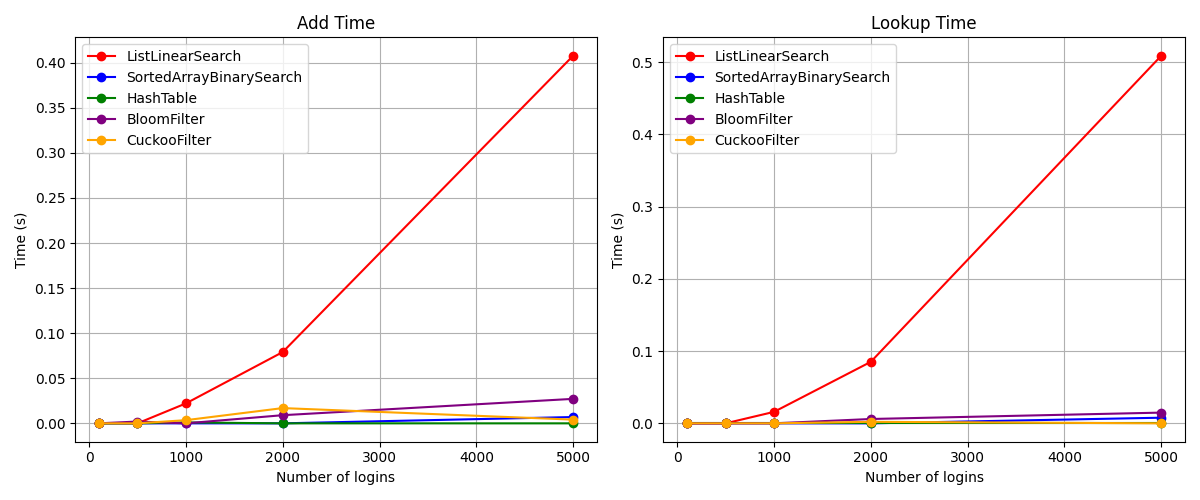
\includegraphics[width=\textwidth]{../img/login_checker_performance.png}
    \caption{Wall-clock performance comparison for all algorithms. Linear search dominates the scale, showing clear quadratic growth for insertions and linear growth for lookups.}
    \label{fig:performance_full}
\end{figure}

Linear search shows dramatic performance degradation (0.49s insertion, 0.57s lookup at $n=5000$), compressing other algorithms into near-flat lines. Figure~\ref{fig:performance_zoomed} provides a zoomed view.

\begin{figure}[h]
    \centering
    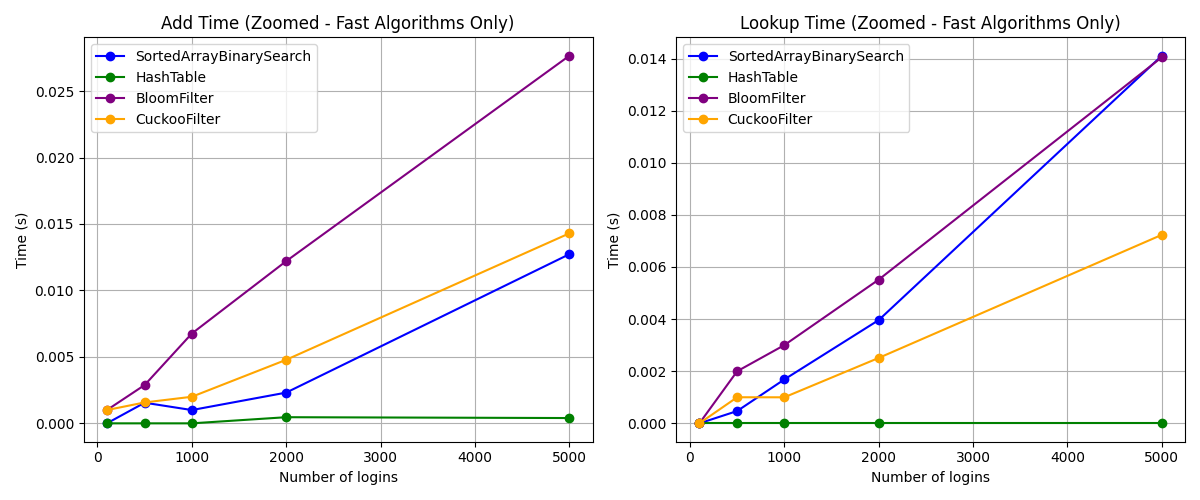
\includegraphics[width=\textwidth]{../img/login_checker_performance_zoomed.png}
    \caption{Zoomed wall-clock performance for efficient algorithms. Hash table maintains near-constant time, while binary search, Bloom filter, and Cuckoo filter show varying degrees of time growth despite theoretical O(log n) and O(1) complexities.}
    \label{fig:performance_zoomed}
\end{figure}


\subsubsection{Theoretical Complexity Validation}

To validate that implementations correctly follow their theoretical complexity, we examine comparison counts rather than wall-clock time. Figure~\ref{fig:comparisons_full} shows average comparisons per operation.

\begin{figure}[h]
    \centering
    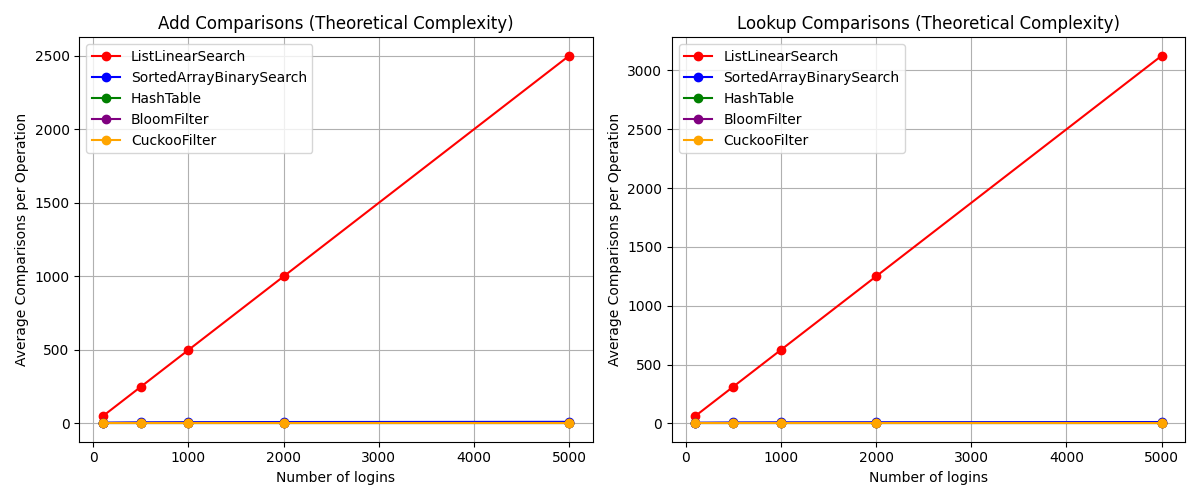
\includegraphics[width=\textwidth]{../img/login_checker_comparisons.png}
    \caption{Average comparison counts per operation. This metric validates theoretical complexity: linear search shows linear growth, binary search shows logarithmic growth, and hash-based approaches show constant comparisons.}
    \label{fig:comparisons_full}
\end{figure}

Comparison counts validate theoretical predictions: linear search shows perfect $O(n)$ growth (50 to 2,500 comparisons), binary search exhibits logarithmic growth (6.4 to 12.2, matching $\log_2(n)$), and hash-based structures maintain constant comparisons ($\sim$1-1.5) regardless of size.

\begin{figure}[h]
    \centering
    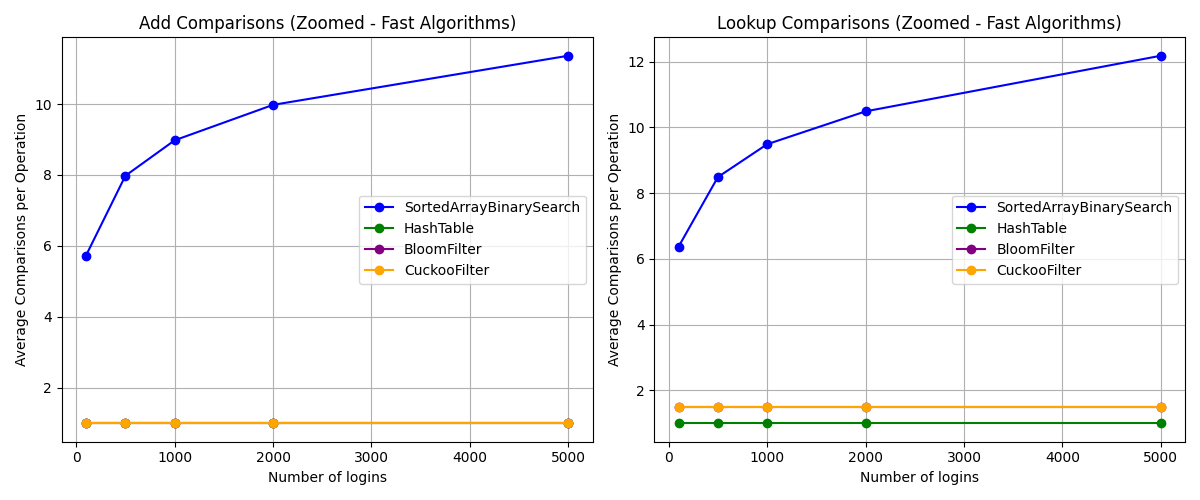
\includegraphics[width=\textwidth]{../img/login_checker_comparisons_zoomed.png}
    \caption{Zoomed comparison counts for efficient algorithms. Binary search exhibits the characteristic logarithmic curve, while hash-based methods remain perfectly flat, validating theoretical predictions.}
    \label{fig:comparisons_zoomed}
\end{figure}

\subsubsection{Key Insights and Analysis}

The dual-metric approach (wall-clock time vs. comparison counts) reveals critical insights about algorithm performance:

\paragraph{Theoretical vs. Practical Performance Gap}

Binary search demonstrates the theory-practice gap: while performing $O(\log n)$ comparisons (12.2 at $n=5000$), wall-clock time grows nearly linearly due to Python string comparison overhead ($\sim$40ns per character across 8.6-character strings). String operations dominate the logarithmic advantage, creating $\sim$800 microseconds per comparison including overhead.

\paragraph{Implementation Overhead in Probabilistic Filters}

While maintaining constant comparisons (validating $O(1)$ theory), Bloom and Cuckoo filters show linear wall-clock growth due to backing set rehashing and library overhead. At $n=5000$: Bloom filter insertion takes 27.7ms vs. 1.0ms for pure hash table; Cuckoo filter performs better (12ms) but still grows linearly.

\paragraph{Hash Table as the Optimal Choice}

Python's native hash table (\texttt{set}) demonstrates genuine $O(1)$ behavior in both comparison counts and wall-clock time, with minimal overhead and near-flat performance across all dataset sizes.

\paragraph{When Simpler Approaches Make Sense}

Despite poor scaling, linear/binary search remain viable for small datasets ($n < 100$), memory-constrained environments, or when sorted access is required.

\paragraph{The Value of Empirical Validation}

Theoretical complexity analysis guides scalability understanding, but constant factors and implementation overhead can dominate practical performance. Comparison counts validate theoretical correctness; wall-clock measurements expose real-world constraints. Both perspectives are necessary for informed algorithm selection.
